% !TEX program = pdflatex
\documentclass[twocolumn, 10pt]{article}
\usepackage[margin=0.75in]{geometry}

% --- PACKAGES ---
\usepackage{amsmath}
\let\Bbbk\relax
\usepackage{amssymb}
\usepackage{booktabs}
\usepackage{graphicx}
\usepackage{url}
\usepackage{algorithm}
\usepackage{algpseudocode}
\usepackage{subcaption}
\usepackage{siunitx}
\usepackage{multirow}

% --- GRAPHICS PATH ---
\graphicspath{{figures/}}

% --- TIKZ & GRAPHICS SETUP ---
\usepackage{tikz}
\usetikzlibrary{arrows.meta, positioning, shapes.geometric, calc, backgrounds, fit, patterns}

% --- COLOR DEFINITIONS ---
\definecolor{Garnet}{HTML}{73000A}
\definecolor{CSecondaryRed}{HTML}{CC2E40}
\definecolor{CBlue}{HTML}{466A9F}
\definecolor{CDark}{HTML}{1F414D}
\definecolor{COlive}{HTML}{65780B}
\definecolor{CLime}{HTML}{CED318}
\definecolor{CGold}{HTML}{A49137}

% --- PLACEHOLDER COMMAND ---
\newcommand{\ph}[1]{\textbf{[#1]}}

\title{A Multi-Mode Simulation Framework for X-Band Pulse Compression Radar}

\author{J.C. Vaught, Douglas Cahl, Yi Wang\\
\small Department of Mechanical Engineering, University of South Carolina, Columbia, SC, 29208}

\begin{document}

\maketitle

\begin{abstract}
Robust radar-based perception for unmanned surface vehicles (USVs) operating in inland and coastal waterways requires large volumes of labeled training data that are logistically difficult, expensive, and time-consuming to collect. We present a multi-mode simulation framework for X-band pulse compression radar designed to address this data scarcity. The framework comprises three generation modes ordered by their role in the algorithm development workflow: (1)~a data-driven compositor that blends synthetic target signatures into real radar recordings, preserving authentic sensor noise and clutter texture for direct use as training data; (2)~an analytical generator using statistical clutter models and stochastic target representations for rapid prototyping of detection parameters; and (3)~an electromagnetic ray-tracing engine for physics-grounded validation of scattering and multipath assumptions. We demonstrate the framework using data from a shore-based Furuno DRS4D~NXT solid-state radar collecting over inland lakes and a coastal harbor in South Carolina. A YOLO-based object detector trained exclusively on Mode~1 composite data achieves \ph{mAP@0.5} on real radar frames containing recreational boats and navigational buoys. We further show that augmenting synthetic training data with real interference and rain-clutter textures improves detector robustness under degraded conditions. The multi-mode architecture enables controlled studies of clutter rejection, object identification, and intermittent-return tracking through configurable scene geometry, sensor parameters, and environmental conditions.
\end{abstract}

%% ============================================================
\section{Introduction}
\label{sec:intro}
%% ============================================================

Unmanned surface vehicles are increasingly deployed for environmental monitoring, hydrographic survey, and infrastructure inspection in inland and coastal waterways~\cite{han2023maritime}. Safe autonomous navigation in these environments demands reliable detection and tracking of other vessels, navigational aids, and obstacles using onboard sensors. X-band marine radar is a natural choice: it provides all-weather, day-night situational awareness at ranges relevant to collision avoidance, and commercial-off-the-shelf (COTS) units are compact, affordable, and field-proven~\cite{skolnik2001introduction}.

Modern detection and tracking pipelines---particularly those built on deep learning---require large quantities of labeled data to generalize across target types, environmental conditions, and clutter regimes~\cite{nikolenko2021synthetic}. Collecting such datasets with accurate ground truth is expensive: it requires instrumented targets, cooperative GPS logging or AIS correlation, and repeated deployments across varying weather and traffic conditions. For small recreational vessels and navigational buoys---targets with low and highly variable radar cross sections (RCS)---the problem is acute because these objects produce intermittent returns that are easily confused with clutter~\cite{ward2013sea, swerling1960probability}.

Synthetic data generation offers a path forward. In the computer vision community, training on synthetic images followed by domain transfer to real sensors has become routine~\cite{tobin2017domain, tremblay2018training}. Analogous efforts for radar remain less developed, particularly for navigation-band marine radar operating at close range over inland waterways.

This paper presents a multi-mode simulation framework for X-band pulse compression radar that generates synthetic training and validation data at three levels of abstraction. Unlike a traditional multi-fidelity hierarchy ordered by physics resolution, the modes are organized by their role in the algorithm development workflow:

\begin{enumerate}
    \item \textbf{Mode~1 --- Data-Driven Compositor.} Blends synthetic target signatures into real radar recordings, producing training data that inherits the authentic noise floor, clutter texture, and sensor artifacts of the physical radar. This mode directly supports supervised learning pipelines.
    \item \textbf{Mode~2 --- Analytical Generator.} Uses parametric clutter and target models to synthesize complete radar frames from statistical first principles, enabling rapid exploration of detection thresholds and algorithm parameters without requiring real data.
    \item \textbf{Mode~3 --- Electromagnetic Ray Tracing.} Simulates pulse-level interactions with 3D scene geometry including material-dependent scattering and multipath propagation, providing physics-grounded reference data for validating assumptions made in Modes~1 and~2.
\end{enumerate}

The framework is demonstrated using data collected with a Furuno DRS4D~NXT solid-state radar installed at fixed shore-based positions overlooking inland lakes and a coastal harbor in South Carolina. We show that a YOLO object detector trained exclusively on Mode~1 composite data transfers effectively to real radar frames, and that augmenting the synthetic training set with real-world degradation patterns (radar interference, rain clutter) further improves robustness.

The contributions of this work are:
\begin{itemize}
    \item A multi-mode synthetic data framework tailored to COTS marine radar operating in inland and littoral environments;
    \item Demonstration that composite synthetic data (Mode~1) enables effective domain transfer for deep-learning-based object detection on real X-band radar data;
    \item An augmentation strategy using real interference and rain-clutter textures to harden detector performance under degraded conditions;
    \item Detailed characterization of the Furuno DRS4D~NXT radar as a research sensor, including data format, resolution, and operating parameters relevant to reproducibility.
\end{itemize}

%% ============================================================
\section{Related Work}
\label{sec:related}
%% ============================================================

\subsection{Synthetic Data for Sensor Perception}

The use of synthetic data to train perception models has been widely studied in computer vision~\cite{tobin2017domain, tremblay2018training, nikolenko2021synthetic}. Domain randomization---varying textures, lighting, and object placement in simulation---has proven effective at closing the sim-to-real gap for camera-based object detection. Analogous approaches exist for lidar point clouds in autonomous driving. For radar, synthetic data generation is less mature, with most published work focusing on synthetic aperture radar (SAR) imagery rather than navigation-band marine radar.

\subsection{Sea and Inland-Water Clutter Modeling}

Statistical models for radar backscatter from water surfaces are well established. The compound K-distribution is the standard model for X-band sea clutter, capturing the heavy-tailed amplitude statistics that arise from the interaction of Bragg scattering with longer-period surface modulation~\cite{ward2013sea, watts1987radar, farina1997high}. Haykin et al.~\cite{haykin2002uncovering} demonstrated the nonlinear dynamical structure in sea clutter time series. These models, developed primarily for open-ocean conditions, provide the statistical foundation for Mode~2 of the framework. Inland waterways, however, present a distinct clutter environment: wave action is wind-driven with no swell component, and fixed clutter from shorelines, docks, and vegetation creates a heterogeneous background that is not well characterized by ocean clutter models alone.

\subsection{Marine Radar Object Detection}

Object detection in marine radar imagery has historically relied on constant false alarm rate (CFAR) processors~\cite{rohling1983radar, gandhi1988analysis}. More recently, deep learning approaches---including YOLO, Faster R-CNN, and transformer-based detectors---have been applied to radar plan position indicator (PPI) images with promising results~\cite{prasad2017object}. These methods require labeled datasets that are scarce for marine radar, particularly in inland settings~\cite{cheng2021robust}. The present work addresses this gap by generating labeled training data synthetically.

\subsection{USV Perception}

Autonomous collision avoidance for USVs is a growing research area~\cite{han2023maritime}. Most published perception systems for USVs rely on cameras, lidar, or AIS transponder data. Radar-based perception for USVs operating in inland waterways---where targets are small, intermittent, and mixed with shore clutter---remains underexplored. This work targets that specific operational regime.

%% ============================================================
\section{Sensor Platform and Data Collection}
\label{sec:sensor}
%% ============================================================

\subsection{Furuno DRS4D NXT Radar}

All data in this study were collected using a Furuno DRS4D~NXT solid-state pulse compression radar. Table~\ref{tab:radar_specs} summarizes the key operating parameters.

\begin{table}[htb]
\centering
\caption{Furuno DRS4D NXT radar specifications.}
\label{tab:radar_specs}
\begin{tabular}{@{}ll@{}}
\toprule
\textbf{Parameter} & \textbf{Value} \\
\midrule
Transmitter type & Solid-state, pulse compression \\
Frequency & \SIrange{9380}{9440}{\mega\hertz} (X-band) \\
Output power & \SI{100}{\watt} \\
Modulation & LFM chirp (Q0N) / unmodulated (P0N) \\
Chirp pulse width & \SIrange{5.0}{18}{\micro\second} (range-dependent) \\
Range resolution & $\sim$\SI{20}{\meter} \\
Horiz.\ beamwidth & \SI{3.9}{\degree} (RezBoost disabled) \\
Vert.\ beamwidth & \SIrange{22}{25}{\degree} \\
Rotation rate & 24 / 36 / 48~RPM (range-coupled) \\
PRF & \SIrange{700}{1100}{\hertz} \\
Azimuth quantization & 8{,}192 spokes per revolution \\
Radome diameter & \SI{610}{\milli\meter} (24~in) \\
\bottomrule
\end{tabular}
\end{table}

The DRS4D~NXT is a Doppler-capable unit, but we operate it with its RezBoost beam-sharpening feature disabled. RezBoost applies a digital deconvolution of the antenna pattern to narrow the effective azimuth beamwidth from \SI{3.9}{\degree} to \SI{2.0}{\degree}; however, this processing can suppress weak target returns. To preserve all detectable echoes---particularly from low-RCS recreational vessels---we retain the native beam pattern throughout data collection.

\subsection{Data Acquisition}

The radar transmits echo data over Ethernet as UDP multicast packets containing spoke-format intensity data. Each spoke represents a one-dimensional array of range-binned echo amplitudes at a specific azimuth angle. The intensity values are log-detected (non-coherent) and represent pre-processed amplitude after internal pulse compression; no in-phase/quadrature (I/Q) data are available at this interface. The data are captured in B-scan (polar) format---a two-dimensional matrix of azimuth versus range---which can be scan-converted to PPI imagery for display or analysis.

\subsection{Collection Campaign}

Data were collected from fixed shore-based installations at three locations in South Carolina over a period of approximately eleven months (January--November 2025). Table~\ref{tab:collections} summarizes the collection campaign.

\begin{table}[htb]
\centering
\caption{Data collection summary.}
\label{tab:collections}
\begin{tabular}{@{}llll@{}}
\toprule
\textbf{Location} & \textbf{Sessions} & \textbf{Range Scale} & \textbf{Conditions} \\
\midrule
Lake Murray, SC & $\sim$\ph{XX} & 0.25--0.75~NM & Fair weather, 1--2 rain events \\
Lake Greenwood, SC & $\sim$\ph{XX} & 0.25--0.75~NM & Fair weather \\
Charleston Harbor, SC & 2--3 & 0.25--0.75~NM & Traffic, radar interference \\
\midrule
\multicolumn{2}{@{}l}{\textbf{Total sessions:} $\sim$30} & \multicolumn{2}{l}{\textbf{Total frames:} $>$\ph{XXX},000} \\
\bottomrule
\end{tabular}
\end{table}

The radar antenna was mounted at heights of \SIrange{2}{4}{\meter} above the water surface, depending on site infrastructure. At these heights and the operational range scales used, the grazing angle is extremely low. For example, at \SI{3}{\meter} height and \SI{0.5}{NM} ($\approx$\SI{926}{\meter}) range:
\begin{equation}
\psi = \arctan\!\left(\frac{h}{R}\right) = \arctan\!\left(\frac{3}{926}\right) \approx 0.19^{\circ}
\label{eq:grazing}
\end{equation}
At such grazing angles, multipath propagation between the direct and water-surface-reflected paths creates constructive and destructive interference lobes. Targets moving through these lobes experience fluctuating received power, producing the intermittent detections that motivate robust tracking algorithms.

The inland lake environments are characterized by minimal wave action---primarily wind-driven chop with no swell---and heterogeneous fixed clutter from shorelines, docks, moored vessels, and vegetation. Charleston Harbor provides a contrasting environment with vessel traffic, tidal currents, and co-channel radar interference from nearby commercial installations.

Targets of interest include recreational powerboats (15--25~ft fiberglass and aluminum hulls), pontoon boats, and navigational buoys. At X-band, fiberglass recreational boats exhibit RCS values of approximately \SIrange{0.5}{20}{\meter\squared} depending on aspect angle, while aluminum vessels and buoys with radar reflectors produce more stable returns in the range of \SIrange{1}{50}{\meter\squared}~\cite{knott2004radar, skolnik2001introduction}.

%% ============================================================
\section{System Architecture}
\label{sec:architecture}
%% ============================================================

The framework provides three distinct modes for generating synthetic radar data, each targeting a different stage of the perception algorithm development cycle. Figure~\ref{fig:architecture} illustrates the overall architecture and data flow.

\begin{figure}[htb]
\centering
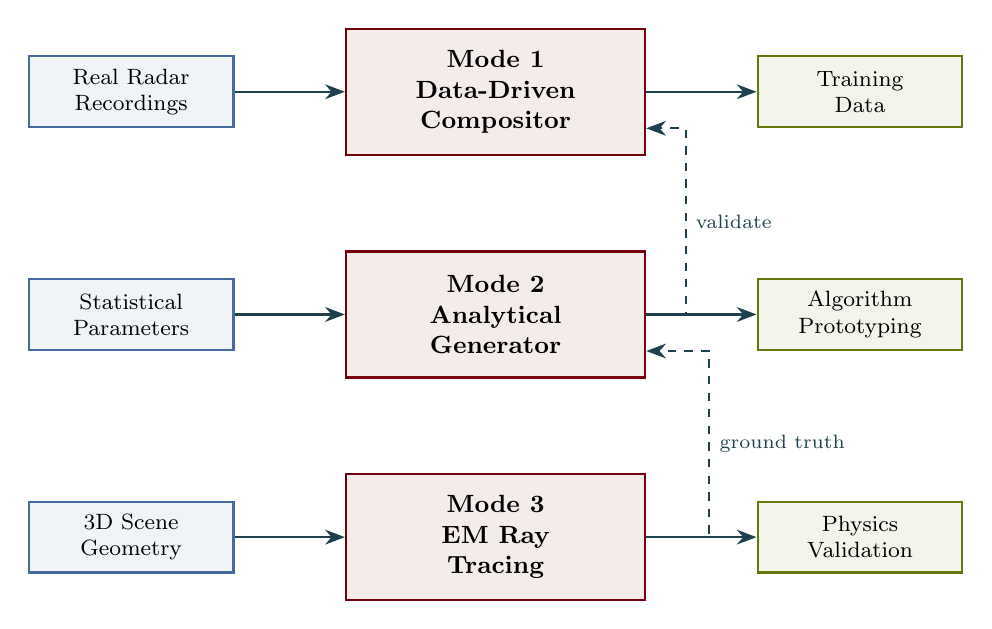
\begin{tikzpicture}[
    node distance=0.8cm and 1.2cm,
    mode/.style={rectangle, draw=Garnet, fill=Garnet!8, thick, minimum width=3.8cm, minimum height=1.6cm, align=center, font=\small\bfseries},
    data/.style={rectangle, draw=CBlue, fill=CBlue!8, thick, minimum width=2.6cm, minimum height=0.9cm, align=center, font=\footnotesize},
    output/.style={rectangle, draw=COlive, fill=COlive!8, thick, minimum width=2.6cm, minimum height=0.9cm, align=center, font=\footnotesize},
    arrow/.style={-{Stealth[length=2.5mm]}, thick, CDark},
    dasharrow/.style={-{Stealth[length=2.5mm]}, thick, CDark, dashed},
]

% Modes
\node[mode] (m1) {Mode 1\\Data-Driven\\Compositor};
\node[mode, below=1.2cm of m1] (m2) {Mode 2\\Analytical\\Generator};
\node[mode, below=1.2cm of m2] (m3) {Mode 3\\EM Ray\\Tracing};

% Inputs
\node[data, left=1.4cm of m1] (real) {Real Radar\\Recordings};
\node[data, left=1.4cm of m2] (params) {Statistical\\Parameters};
\node[data, left=1.4cm of m3] (scene) {3D Scene\\Geometry};

% Outputs
\node[output, right=1.4cm of m1] (train) {Training\\Data};
\node[output, right=1.4cm of m2] (proto) {Algorithm\\Prototyping};
\node[output, right=1.4cm of m3] (valid) {Physics\\Validation};

% Arrows
\draw[arrow] (real) -- (m1);
\draw[arrow] (params) -- (m2);
\draw[arrow] (scene) -- (m3);
\draw[arrow] (m1) -- (train);
\draw[arrow] (m2) -- (proto);
\draw[arrow] (m3) -- (valid);

% Cross-mode arrows
\draw[dasharrow] (m2.east) -- ++(0.5,0) |- node[right, pos=0.25, font=\scriptsize, text=CDark]{validate} (m1.east |- train.south);
\draw[dasharrow] (m3.east) -- ++(0.8,0) |- node[right, pos=0.25, font=\scriptsize, text=CDark]{ground truth} (m2.east |- proto.south);

\end{tikzpicture}
\caption{Multi-mode framework architecture. Solid arrows indicate primary data flow; dashed arrows indicate cross-mode validation pathways. Modes are ordered by workflow utility: Mode~1 produces production training data, Mode~2 enables rapid parameter exploration, and Mode~3 provides physics-grounded reference.}
\label{fig:architecture}
\end{figure}

The three modes share a common world model that defines the scene geometry: radar position and height, water surface, target positions and trajectories, and fixed clutter objects (shorelines, docks). This shared representation ensures that equivalent scenarios can be instantiated across modes for cross-validation.

%% ============================================================
\section{Mode 1: Data-Driven Compositor}
\label{sec:mode1}
%% ============================================================

Mode~1 generates training data by compositing synthetic target signatures into real radar recordings. This approach inherits the authentic noise floor, clutter texture, and sensor artifacts present in the real data while providing complete control over target placement, quantity, and labeling.

\subsection{Compositing Pipeline}

The compositing process operates on B-scan (polar-format) radar frames and proceeds as follows:

\begin{enumerate}
    \item \textbf{Background selection.} A real radar frame is selected from the recording database. Frames may be chosen based on environmental conditions (calm, rain, interference) or clutter characteristics.
    \item \textbf{Target signature generation.} A synthetic target return is generated based on a parametric model of the target's radar cross section, range, and azimuth extent. The target signature accounts for the radar's range resolution, azimuth beamwidth, and the expected amplitude distribution for the target class.
    \item \textbf{Amplitude matching.} The synthetic target intensity is scaled to be consistent with the local clutter statistics of the insertion region, ensuring that the signal-to-clutter ratio (SCR) is physically plausible for the specified target RCS and range.
    \item \textbf{Insertion and blending.} The target signature is inserted into the B-scan frame. \ph{Describe your specific blending method---additive? replacement? weighted? Do you apply any spatial smoothing at the boundary?}
    \item \textbf{Label generation.} Bounding box annotations are automatically generated for each inserted target in the format required by the downstream detector (e.g., YOLO-format normalized coordinates).
\end{enumerate}

\subsection{Environmental Augmentation}

A key advantage of Mode~1 is the ability to augment training data with real-world degradation patterns extracted from the recording database:

\begin{itemize}
    \item \textbf{Radar interference.} Co-channel interference from nearby marine radars produces characteristic radial spoke artifacts in the B-scan. Interference patterns captured at Charleston Harbor are extracted and composited onto clean training frames at varying intensities.
    \item \textbf{Rain clutter.} Precipitation produces spatially correlated, diffuse returns that elevate the noise floor across range-azimuth cells. Rain-clutter textures captured during collection are blended into synthetic frames.
\end{itemize}

These augmentations expose the detector to degraded conditions during training without requiring additional field collections under those specific conditions.

%% ============================================================
\section{Mode 2: Analytical Generator}
\label{sec:mode2}
%% ============================================================

Mode~2 synthesizes complete radar frames from parametric statistical models, enabling rapid exploration of detection algorithm parameters without requiring real data.

\subsection{Clutter Model}

The amplitude statistics of radar backscatter from the water surface are modeled using the compound K-distribution~\cite{ward2013sea, watts1987radar}. The probability density function of the echo envelope $x$ is given by:
\begin{equation}
f(x) = \frac{4}{\Gamma(\nu)} \left(\frac{\nu}{P_c}\right)^{\!\frac{\nu+1}{2}} x^{\nu}\, K_{\nu-1}\!\left(2\sqrt{\frac{\nu\, x^2}{P_c}}\right), \quad x \geq 0
\label{eq:kdist}
\end{equation}
where $\nu$ is the shape parameter controlling the tail behavior (smaller $\nu$ implies heavier tails and spikier clutter), $P_c$ is the mean clutter power, $\Gamma(\cdot)$ is the gamma function, and $K_{\nu-1}(\cdot)$ is the modified Bessel function of the second kind. For the calm inland lake conditions that dominate our dataset, $\nu$ is expected to be relatively large (approaching Rayleigh statistics), reflecting the absence of long-period sea-surface modulation.

\subsection{Target Model}

Targets are modeled as fluctuating point scatterers with RCS drawn from a Swerling~I distribution (scan-to-scan fluctuation, exponential PDF)~\cite{swerling1960probability}. The received target power at range $R$ follows the radar equation:
\begin{equation}
P_r = \frac{P_t\, G^2\, \lambda^2\, \sigma}{(4\pi)^3\, R^4\, L}
\label{eq:radarequation}
\end{equation}
where $P_t$ is the transmit power, $G$ is the antenna gain, $\lambda$ is the wavelength, $\sigma$ is the target RCS, and $L$ accounts for system losses. The target return is spread across range and azimuth bins according to the radar's point spread function (range resolution and antenna beam pattern).

\subsection{Frame Synthesis}

A synthetic B-scan frame is generated by:
\begin{enumerate}
    \item Drawing a clutter realization from the K-distribution for each range-azimuth cell, with parameters that may vary spatially to represent shore clutter zones versus open water;
    \item Adding target returns at specified positions with RCS drawn from the Swerling model;
    \item Applying log-detection to match the amplitude scaling of the real radar data;
    \item Optionally adding thermal noise and interference models.
\end{enumerate}

\ph{Include a figure comparing Mode~2 synthetic clutter amplitude histogram against real data once this validation is complete.}

%% ============================================================
\section{Mode 3: Electromagnetic Ray Tracing}
\label{sec:mode3}
%% ============================================================

Mode~3 provides the highest-fidelity synthetic data by simulating pulse-level electromagnetic interactions with 3D scene geometry. This mode serves as a physics reference for validating assumptions in Modes~1 and~2.

\subsection{Architecture}

The ray-tracing engine employs a shooting-and-bouncing-rays (SBR) approach~\cite{ling1989shooting} adapted for the marine radar geometry. For each transmitted pulse:
\begin{enumerate}
    \item Rays are launched from the radar antenna according to the beam pattern;
    \item Rays propagate through the scene, intersecting with the water surface and target geometry;
    \item At each intersection, reflected and scattered rays are generated based on material properties and surface roughness;
    \item Rays returning to the radar aperture are coherently summed to produce the received signal;
    \item The received signal is match-filtered (pulse compression) and log-detected to produce the intensity value for each range bin.
\end{enumerate}

The water surface is modeled as a time-varying mesh whose elevation profile is generated from a wind-driven wave spectrum. At the low grazing angles encountered in our geometry ($\psi < 1^{\circ}$), multipath between the direct path and the specular reflection off the water surface creates an interference pattern that modulates target visibility as a function of range~\cite{long2001radar, blake1986radar}.

\subsection{Current Status}

The ray-tracing engine is functional for canonical validation scenarios---single targets over a flat or gently perturbed water surface---but does not yet incorporate the full scene complexity (shoreline geometry, vegetation, dock structures) present in the inland lake environment. Extension to these heterogeneous scenes is ongoing. Preliminary validation against the two-ray (Lloyd's mirror) multipath model shows agreement in the interference lobe structure for point targets at ranges of \SIrange{100}{1000}{\meter}.

%% ============================================================
\section{Results}
\label{sec:results}
%% ============================================================

\subsection{Mode 1: Domain Transfer for Object Detection}

To evaluate whether synthetic training data from Mode~1 enables effective object detection on real radar data, we trained a YOLOv\ph{X} detector~\cite{jocher2023yolov8} exclusively on Mode~1 composite frames and evaluated it on held-out real radar recordings.

\subsubsection{Training Configuration}

\begin{itemize}
    \item \textbf{Training data:} \ph{N} composite B-scan frames generated by Mode~1, containing \ph{describe: how many targets per frame? what target classes? boats only, or boats+buoys?}
    \item \textbf{Annotations:} Automatically generated bounding boxes for all inserted targets
    \item \textbf{Model:} YOLOv\ph{X} with \ph{describe: what backbone? what input size? any modifications?}
    \item \textbf{Training:} \ph{N} epochs, \ph{batch size}, \ph{optimizer}, \ph{learning rate}
    \item \textbf{No real data were used during training.}
\end{itemize}

\subsubsection{Evaluation on Real Data}

The trained model was evaluated on \ph{N} real radar frames containing \ph{N} annotated targets (recreational boats and buoys) from \ph{which locations?}. Table~\ref{tab:yolo_results} reports detection performance.

\begin{table}[htb]
\centering
\caption{Object detection performance: Mode~1 synthetic training evaluated on real data.}
\label{tab:yolo_results}
\begin{tabular}{@{}lcccc@{}}
\toprule
\textbf{Training Data} & \textbf{Precision} & \textbf{Recall} & \textbf{mAP@0.5} & \textbf{mAP@0.5:0.95} \\
\midrule
Mode 1 (clean) & \ph{X.XX} & \ph{X.XX} & \ph{X.XX} & \ph{X.XX} \\
\bottomrule
\end{tabular}
\end{table}

\ph{Add 1--2 sentences interpreting the results. What works well? Any failure modes?}

\ph{Include a figure showing example detection frames: real radar B-scan/PPI with YOLO bounding boxes overlaid on correctly detected boats/buoys.}

\subsection{Augmented Training: Robustness Under Degraded Conditions}

We evaluated whether augmenting Mode~1 training data with real interference and rain-clutter textures improves detector robustness when tested on real data collected under those conditions.

\subsubsection{Experimental Design}

Five training/test configurations were evaluated, as summarized in Table~\ref{tab:augmentation}.

\begin{table}[htb]
\centering
\caption{Augmentation experiment: mAP@0.5 across training and test conditions.}
\label{tab:augmentation}
\begin{tabular}{@{}llc@{}}
\toprule
\textbf{Training Set} & \textbf{Test Set} & \textbf{mAP@0.5} \\
\midrule
Clean Mode 1 & Clean real & \ph{X.XX} \\
Clean Mode 1 & Rain real & \ph{X.XX} \\
Clean Mode 1 & Interference real & \ph{X.XX} \\
Augmented Mode 1 & Rain real & \ph{X.XX} \\
Augmented Mode 1 & Interference real & \ph{X.XX} \\
\bottomrule
\end{tabular}
\end{table}

The augmented training set was constructed by overlaying \ph{N} interference patterns and \ph{N} rain-clutter textures, extracted from real recordings, onto the existing clean Mode~1 composite frames. The total augmented training set contained \ph{N} frames.

\ph{Add 1--2 sentences interpreting the augmentation results. How much did performance drop on degraded data? How much did augmentation recover?}

\subsection{Mode 1: Compositor Validation}

To verify that composited targets are statistically consistent with the surrounding radar data, we compared the amplitude distribution within insertion regions against adjacent clutter-only regions.

\ph{Describe your validation here. Include: (1)~histogram overlay of composited region vs.\ surrounding clutter, (2)~Kolmogorov--Smirnov test result (test statistic and p-value), (3)~a before/after compositor figure showing the real frame, the composite frame, and the difference.}

\subsection{Computational Performance}

A central design goal of the multi-mode framework is to provide generation speeds appropriate for each stage of the algorithm development workflow. We benchmarked all three modes by generating 100 frames of 720 spokes each on a single workstation. Table~\ref{tab:benchmark} reports the per-frame timing statistics.

\begin{table}[htb]
\centering
\caption{Per-frame generation time for 100 frames of 720 spokes each.}
\label{tab:benchmark}
\begin{tabular}{@{}lS[table-format=3.2]S[table-format=1.4]S[table-format=1.4]S[table-format=1.4]S[table-format=1.4]@{}}
\toprule
\textbf{Mode} & {\textbf{Total (s)}} & {\textbf{Mean (s)}} & {\textbf{Median (s)}} & {\textbf{Min (s)}} & {\textbf{Max (s)}} \\
\midrule
1 --- Compositor   & 26.57  & 0.2657 & 0.2647 & 0.1936 & 0.3409 \\
2 --- Analytical   &  8.08  & 0.0808 & 0.0797 & 0.0751 & 0.1595 \\
3 --- Ray Tracing  & 326.67 & 3.2667 & 3.0528 & 2.9192 & 8.0327 \\
\bottomrule
\end{tabular}
\end{table}

Mode~2 is the fastest generator, producing frames in \SI{81}{\milli\second} on average---approximately 12~frames per second---making it well suited to rapid parameter sweeps and Monte Carlo studies where thousands of frames are needed. Mode~1 averages \SI{266}{\milli\second} per frame (${\sim}$3.8~fps), dominated by the cost of reading the background recording and blending the synthetic signature; this throughput is sufficient for generating training sets of $10^{4}$--$10^{5}$ frames overnight. Mode~3 requires \SI{3.27}{\second} per frame, roughly 40$\times$ slower than Mode~2, reflecting the computational cost of per-spoke ray propagation and coherent summation. While Mode~3 throughput is adequate for producing small validation sets, it is not practical for large-scale training data generation---a deliberate design trade-off that motivates the multi-mode architecture. The standard deviation for Mode~3 (\SI{0.74}{\second}) is notably larger than for the other modes, due to occasional spikes caused by complex multipath geometries that increase the number of ray--surface intersections.

%% ============================================================
\section{Discussion}
\label{sec:discussion}
%% ============================================================

\subsection{Strengths and Limitations of Mode 1}

The compositor approach has a fundamental strength: because it inherits real sensor noise, clutter texture, and artifacts, the synthetic training data is inherently well-matched to the target domain. This minimizes the sim-to-real gap that plagues fully synthetic approaches. The main limitation is that Mode~1 requires real background recordings for every environment of interest. Generating training data for a new waterway or radar installation requires first collecting background data at that site.

\subsection{The Inland Waterway Domain}

The majority of our data were collected over inland lakes, where clutter conditions differ substantially from the open-ocean environments assumed by most sea clutter models~\cite{ward2013sea}. Inland waterways exhibit near-glassy calm conditions punctuated by light wind chop, heterogeneous shoreline returns, and man-made structures. The K-distribution shape parameter $\nu$ for these environments is expected to be large, approaching Rayleigh statistics, but systematic characterization remains ongoing (Mode~2 development). We note that inland-waterway radar perception is underrepresented in the literature relative to open-ocean maritime surveillance, despite the growing deployment of USVs in rivers, lakes, and harbors~\cite{cheng2021robust}.

\subsection{Low Grazing Angle Effects}

At antenna heights of \SIrange{2}{4}{\meter} and operational ranges of \SIrange{0.25}{0.75}{NM}, the grazing angle is below \SI{0.5}{\degree} throughout the scene (Eq.~\ref{eq:grazing}). This extreme geometry causes strong multipath interference: targets fade in and out of detectability as they traverse the constructive and destructive lobes of the two-ray interference pattern~\cite{long2001radar}. This intermittent-return behavior is a primary driver of track fragmentation and motivates the need for training data that captures realistic detection statistics across range and aspect angle.

\subsection{Limitations and Future Work}

\ph{Honest list of what doesn't work or isn't finished. Suggestions:}
\begin{itemize}
    \item Mode~2 analytical generator validation against real clutter statistics is ongoing.
    \item Mode~3 ray tracer does not yet model complex shoreline geometry or vegetation clutter.
    \item The current study is limited to fair-weather inland conditions; extension to higher sea states and open water is planned.
    \item The training/test split uses data from the same collection sites; cross-site generalization has not yet been evaluated.
    \item \ph{Add any other known limitations.}
\end{itemize}

%% ============================================================
\section{Conclusion}
\label{sec:conclusion}
%% ============================================================

We presented a multi-mode simulation framework for X-band pulse compression radar that generates synthetic training and validation data for perception algorithms operating in inland and coastal waterways. The framework comprises three modes organized by workflow utility: a data-driven compositor for production training data, an analytical generator for rapid algorithm prototyping, and an electromagnetic ray tracer for physics validation. Using data from a Furuno DRS4D~NXT radar collected across approximately 30~sessions at inland lakes and a coastal harbor in South Carolina, we demonstrated that a YOLO detector trained exclusively on Mode~1 composite data achieves \ph{mAP@0.5} on real radar frames. Augmenting synthetic training data with real interference and rain-clutter patterns further improves robustness under degraded conditions. The framework provides a controlled, reproducible environment for developing and benchmarking radar-based perception algorithms for unmanned surface vehicles without requiring extensive labeled field collections.

%% ============================================================
\section*{Acknowledgments}
%% ============================================================

\ph{Acknowledge funding sources, lab members, or anyone who helped with data collection.}

%% ============================================================

\bibliographystyle{unsrt}
\bibliography{references}

\end{document}
